
\section{Bedienoberfläche}


\newcounter{gui}\setcounter{gui}{10}

\begin{description}[leftmargin=5em, style=sameline]	
	\begin{lhp}{gui}{GUI}{gui:beispiel}
		\item[Name:] Login
		\item[Beschreibung:] Interface für Anmeldung und neu Registrierung
		\item[Relevante Systemfunktionen:] \ref{funk:zugriff}
		\item[Abbildungen:] \ref{gui:login}
	\end{lhp}
\end{description}

\begin{description}[leftmargin=5em, style=sameline]	
	\begin{lhp}{gui}{GUI}{gui:beispiel}
		\item[Name:] Hauptmenu
		\item[Beschreibung:] Man kann auf verschiedene Untermenus zugreufen, Profil, Spiel gegen Computer, Spiel gegen Freunde, Regeln und Profil löschen.
		\item[Relevante Systemfunktionen:] 
		\ref{funk:zugriff}
		\item[Abbildungen:] \ref{gui:hauptmenu}
	\end{lhp}
\end{description}

\begin{description}[leftmargin=5em, style=sameline]	
	\begin{lhp}{gui}{GUI}{gui:beispiel}
		\item[Name:] Profil und Daten

		\item[Beschreibung:] Man kann ggf. das Passwort ändern oder das ganze Profil löschen. Desweiteren wird die Anzahl der bereits beendeten Spiel, der gewonnenen Spiele und eine Bestenliste .

		\item[Relevante Systemfunktionen:]  \ref{funk:zugriff},\ref{funk:bestenliste} , /LF50/
		\item[Abbildungen:] \ref{gui:profil}
	\end{lhp}
\end{description}

\begin{description}[leftmargin=5em, style=sameline]	
	\begin{lhp}{gui}{GUI}{gui:beispiel}
		\item[Name:] Passwort ändern
		\item[Beschreibung:] Der Spieler kann das Passwort ändern.
		\item[Relevante Systemfunktionen:] \ref{funk:zugriff}
		\item[Abbildungen:] \ref{gui:passworta}
	\end{lhp}
\end{description}

\begin{description}[leftmargin=5em, style=sameline]	
	\begin{lhp}{gui}{GUI}{gui:beispiel}
		\item[Name:] Lobby
		\item[Beschreibung:] Man kann auswählen on man einem bereits erstellten Spielraum beitritt oder einen eigenen Spielraum erstellt.
		\item[Relevante Systemfunktionen:] \ref{funk:spielraum}
		\item[Abbildungen:] \ref{gui:lobby}
	\end{lhp}
\end{description}

\begin{description}[leftmargin=5em, style=sameline]	
	\begin{lhp}{gui}{GUI}{gui:beispiel}
		\item[Name:] Spielraum erstellen
		\item[Beschreibung:] Ein Spieler kann ein Spielraum erstellen und kann optional ein Passwort dafür festlegen. Desweiteren setzt er noch die Anzahl der Spieler fest.
		\item[Relevante Systemfunktionen:] \ref{funk:spielraum}
		\item[Abbildungen:] \ref{gui:erstellung}
	\end{lhp}
\end{description}

\begin{description}[leftmargin=5em, style=sameline]	
	\begin{lhp}{gui}{GUI}{gui:beispiel}
		\item[Name:] Passwort für Spielraum
		\item[Beschreibung:] Falls der ausgewählte Spielraum ein Passwort benötigt, wird dieser hier abgefragt.
		\item[Relevante Systemfunktionen:] \ref{funk:spielraum}
		\item[Abbildungen:] \ref{gui:passwortspielraum}
	\end{lhp}
\end{description}

\begin{description}[leftmargin=5em, style=sameline]	
	\begin{lhp}{gui}{GUI}{gui:beispiel}
		\item[Name:] Warten auf Spieler
		\item[Beschreibung:]  Hier warten die Spieler bis genügend Spieler da sind und Das Spiel gestartet werden kann.
		\item[Relevante Systemfunktionen:] \ref{funk:spielraum}
		\item[Abbildungen:] \ref{gui:wartebereich}
	\end{lhp}
\end{description}

\begin{description}[leftmargin=5em, style=sameline]	
	\begin{lhp}{gui}{GUI}{gui:beispiel}
		\item[Name:] Spielraum 
		\item[Beschreibung:] Man kann mit den andern Spieler in einem Chat schreiben und man kann das Spiel verlassen.
		\item[Relevante Systemfunktionen:] /LF50/ , /LF60/ , /LF70/
		\item[Abbildungen:] \ref{gui:spielbrett}
	\end{lhp}
\end{description}

\begin{description}[leftmargin=5em, style=sameline]	
	\begin{lhp}{gui}{GUI}{gui:beispiel}
		\item[Name:] Regeln
		\item[Beschreibung:] Die Spieler können die Regeln des Spiels nachlesen.
		\item[Relevante Systemfunktionen:] keine
		\item[Abbildungen:] \ref{gui:regeln}
	\end{lhp}
\end{description}

\begin{description}[leftmargin=5em, style=sameline]	
	\begin{lhp}{gui}{GUI}{gui:beispiel}
		\item[Name:] Zusammenhänge
		\item[Beschreibung:] Zusammenhänge zwischen GUI-Ansichten
		\item[Relevante Systemfunktionen:] Alle
		\item[Abbildungen:] \ref{gui:zusammenhang}
	\end{lhp}
\end{description}



\begin{figure}
	\centering
	\includegraphics[width=0.9\textwidth]{img/login}
	\caption{Login}
	\label{gui:login}
\end{figure}

\begin{figure}
	\centering
	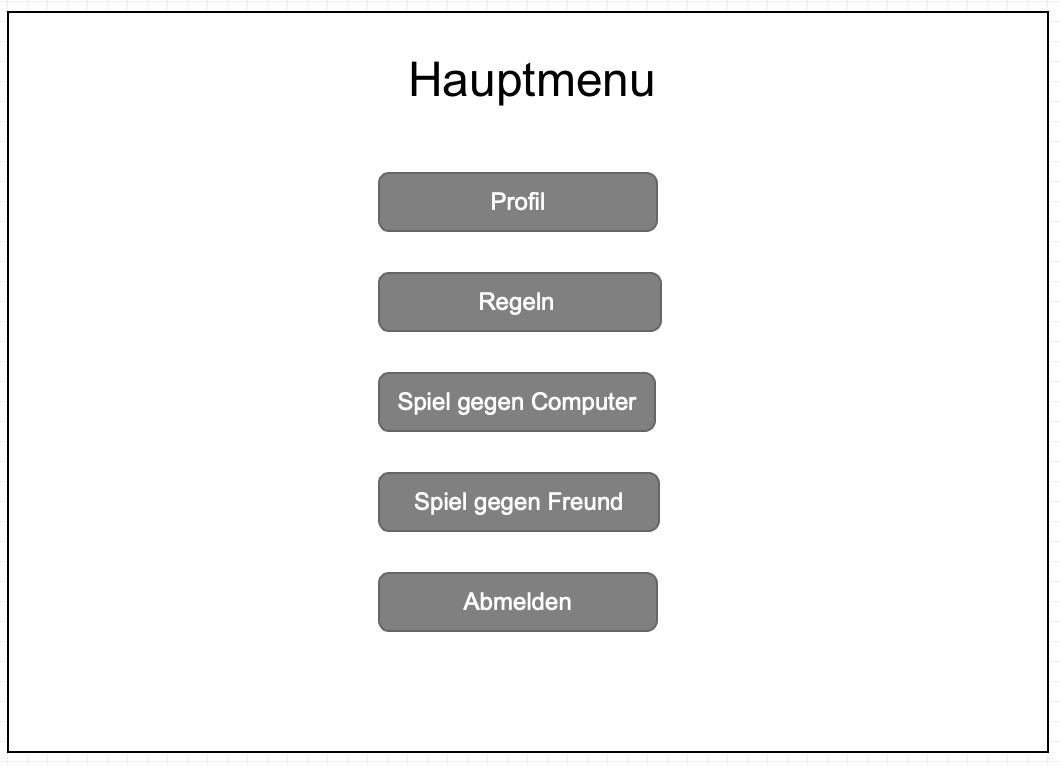
\includegraphics[width=0.9\textwidth]{img/Hauptmenu}
	\caption{Hauptmenu)}
	\label{gui:hauptmenu}
\end{figure}


\begin{figure}
	\centering
	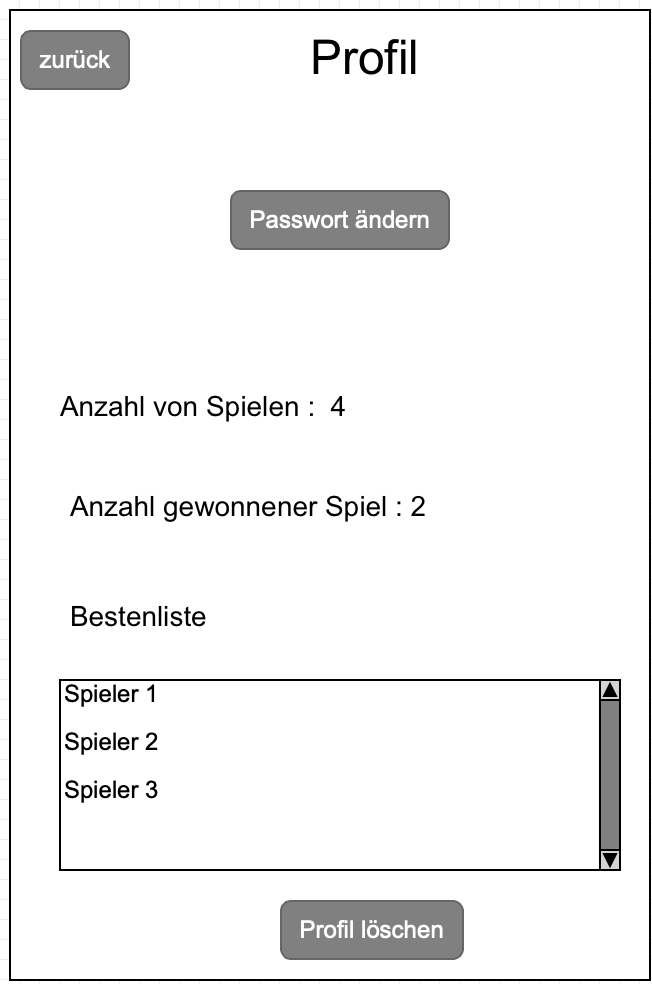
\includegraphics[width=0.9\textwidth]{img/Profil}
	\caption{Profil}
	\label{gui:profil}
\end{figure}

\begin{figure}
	\centering
	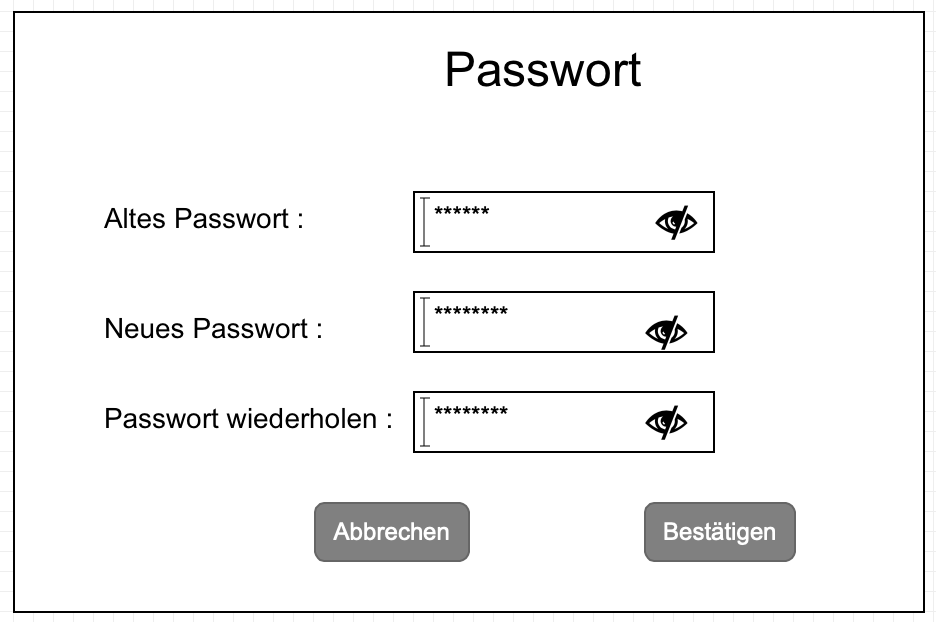
\includegraphics[width=0.9\textwidth]{img/Passwortanderung}
	\caption{Passwort ändern}
	\label{gui:passworta}
\end{figure}


\begin{figure}
	\centering
	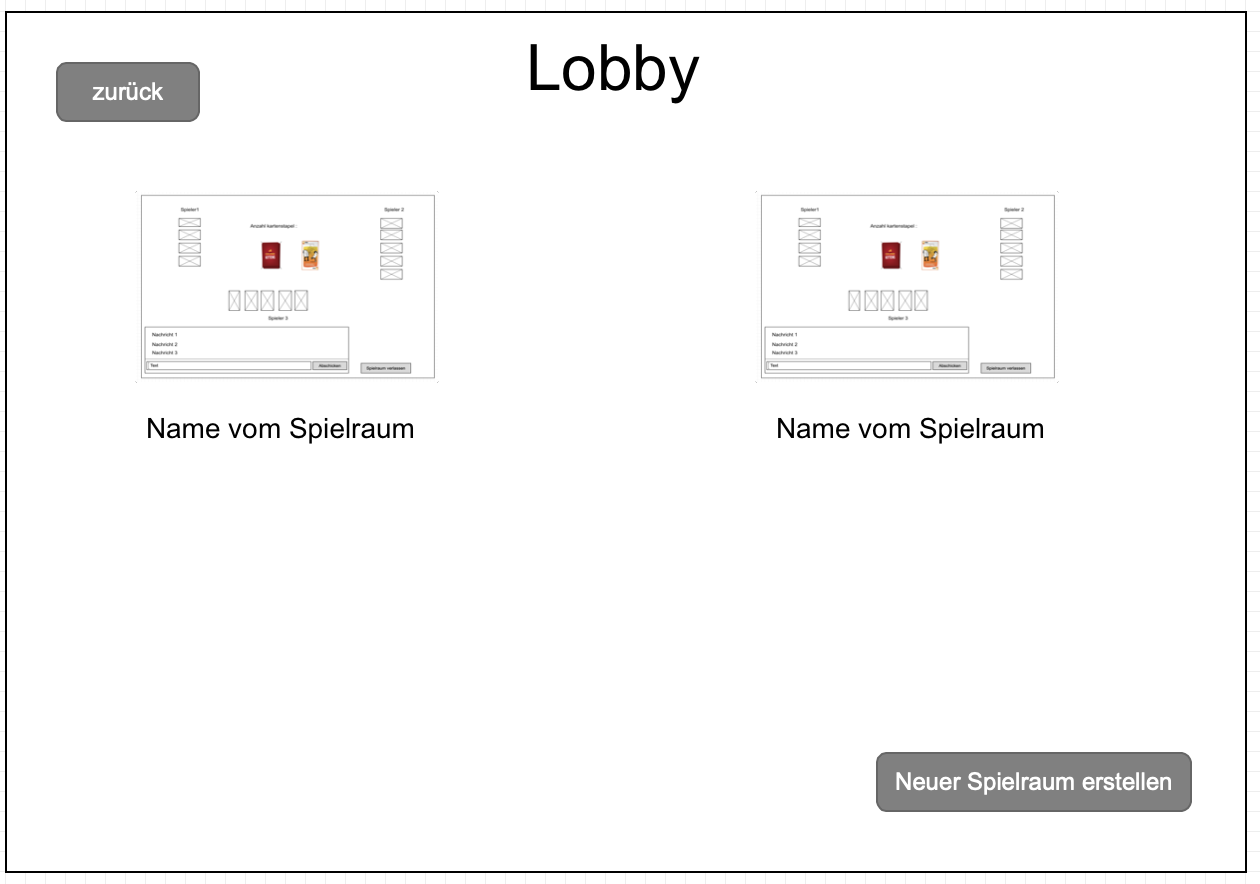
\includegraphics[width=0.9\textwidth]{img/Lobby}
	\caption{Lobby}
	\label{gui:lobby}
\end{figure}

\begin{figure}
	\centering
	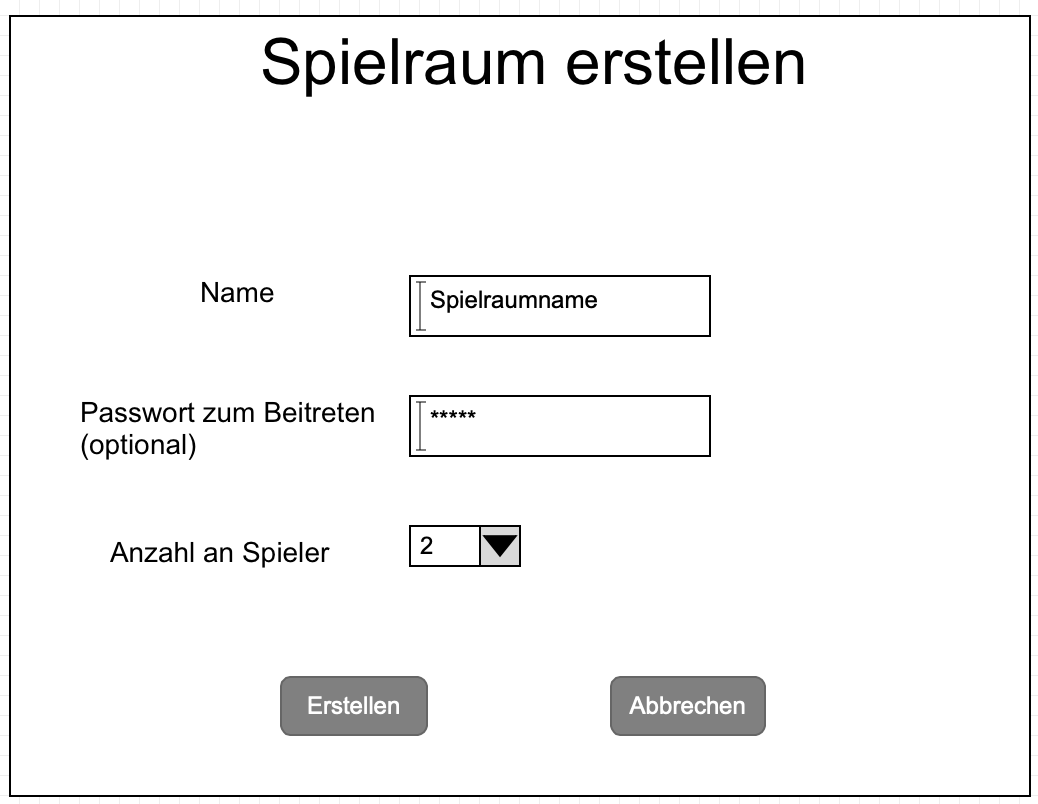
\includegraphics[width=0.9\textwidth]{img/Spielraumerstellen}
	\caption{Spielraum erstellen}
	\label{gui:erstellung}
\end{figure}

\begin{figure}
	\centering
	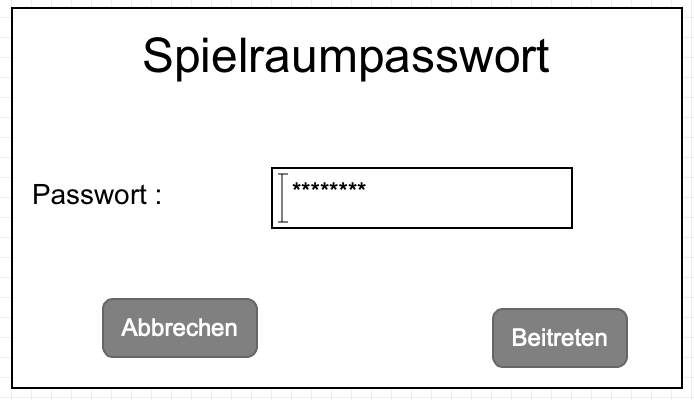
\includegraphics[width=0.9\textwidth]{img/Spielraumpasswort}
	\caption{Passwort für Spielraum}
	\label{gui:passwortspielraum}
\end{figure}

\begin{figure}
	\centering
	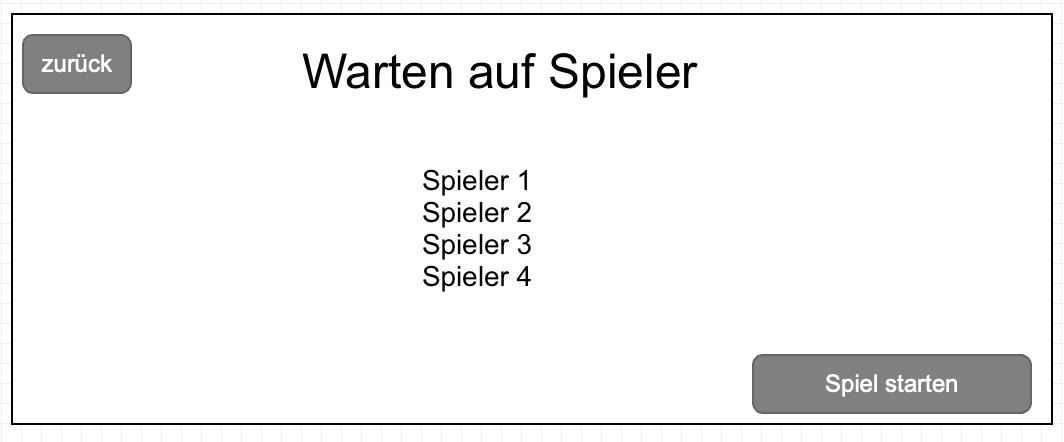
\includegraphics[width=0.9\textwidth]{img/Warten}
	\caption{warten auf Spieler}
	\label{gui:wartebereich}

\end{figure}

\begin{figure}
	\centering
	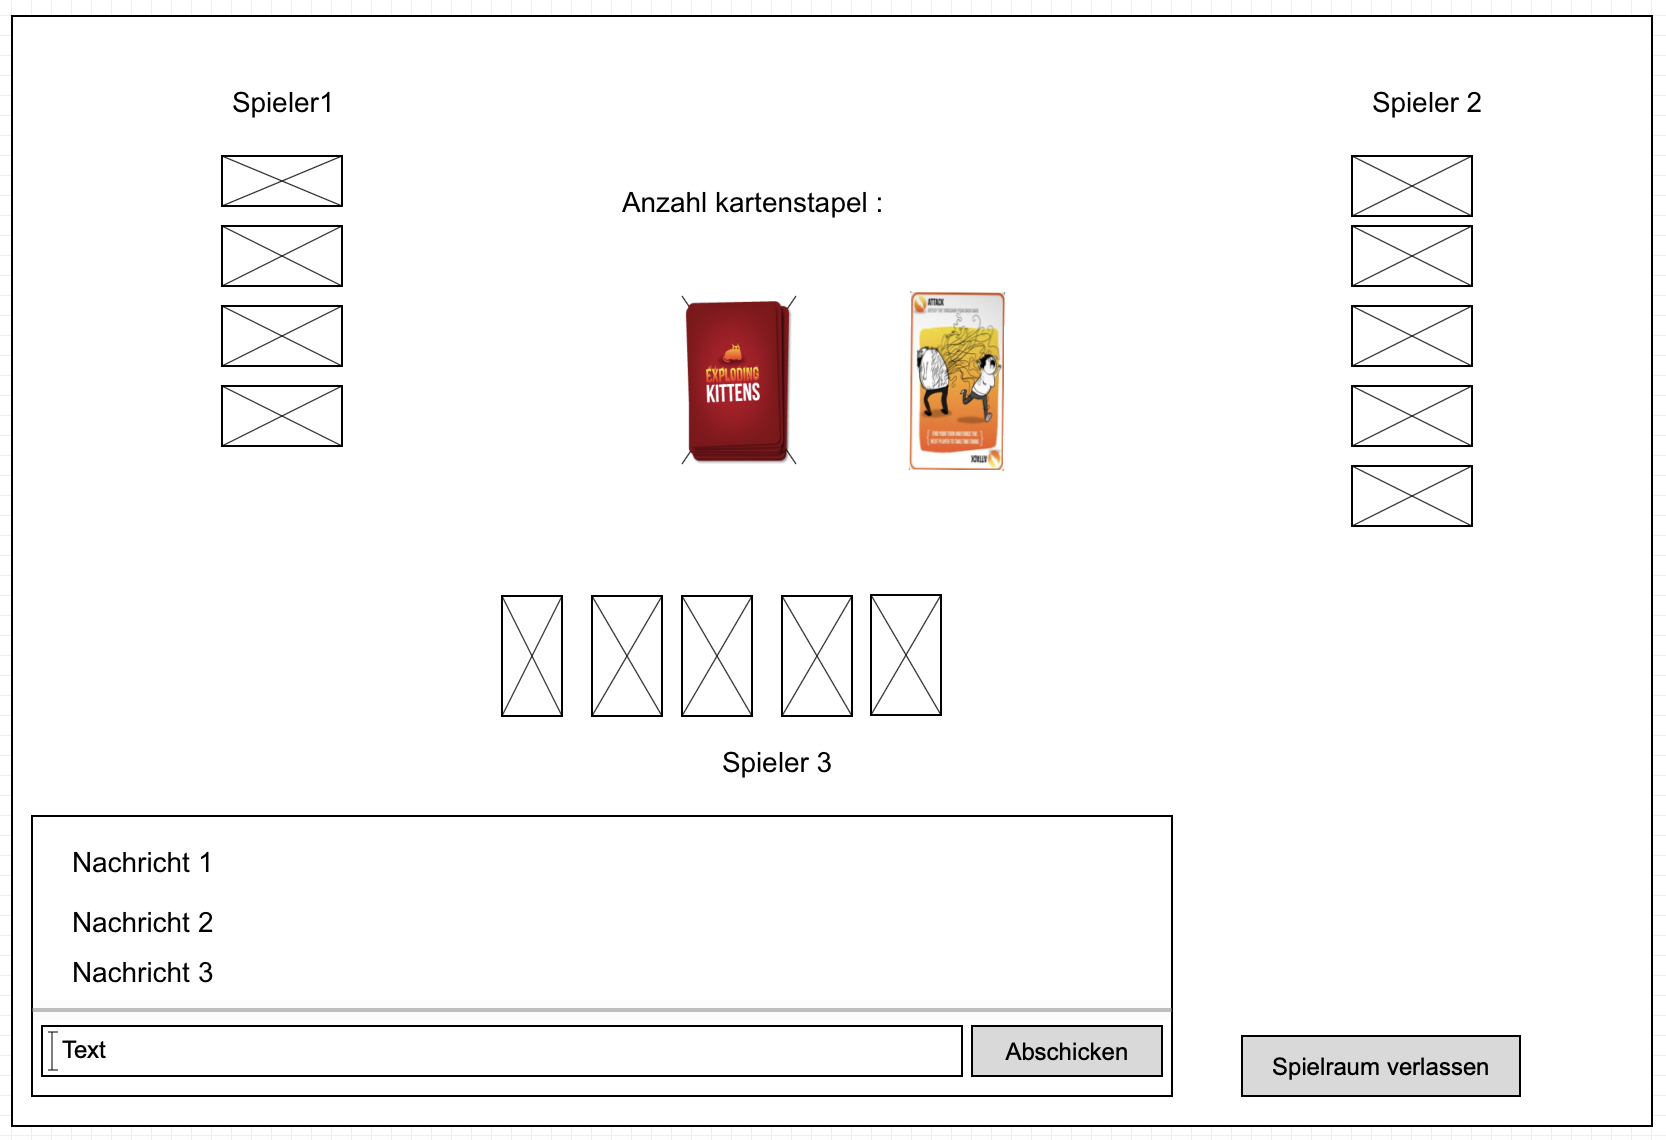
\includegraphics[width=0.9\textwidth]{img/Spielbrett}
	\caption{Spielbraum}
	\label{gui:spielbrett}
\end{figure}

\begin{figure}
	\centering
	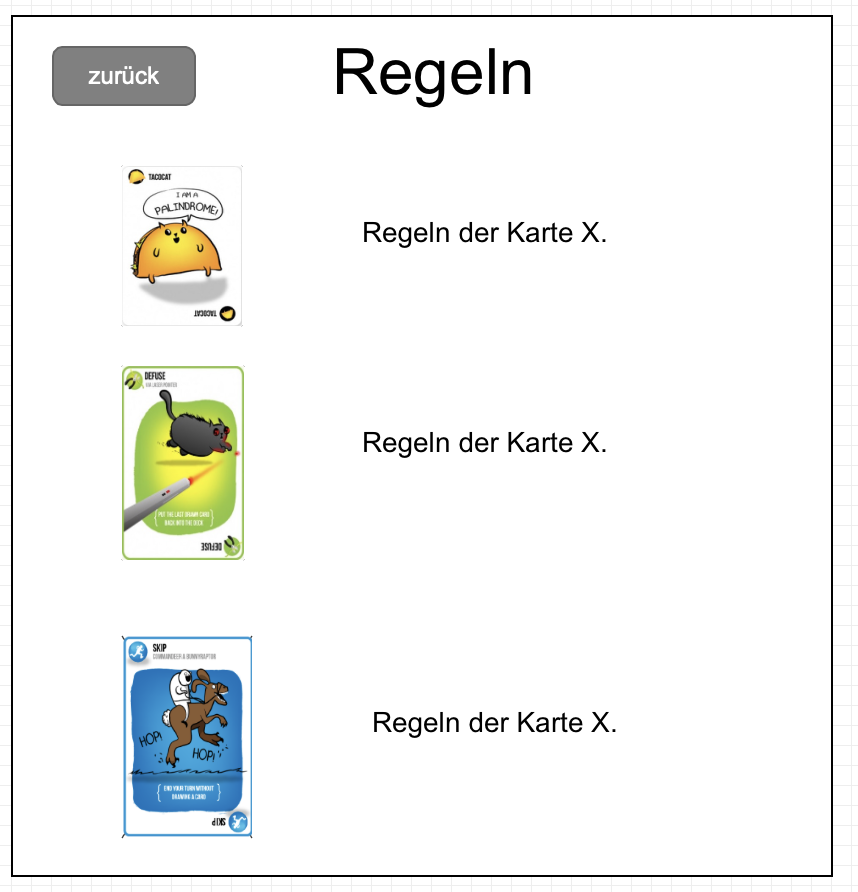
\includegraphics[width=0.9\textwidth]{img/Regeln}
	\caption{Regeln}
	\label{gui:regeln}
\end{figure}


\begin{figure}
	\centering
	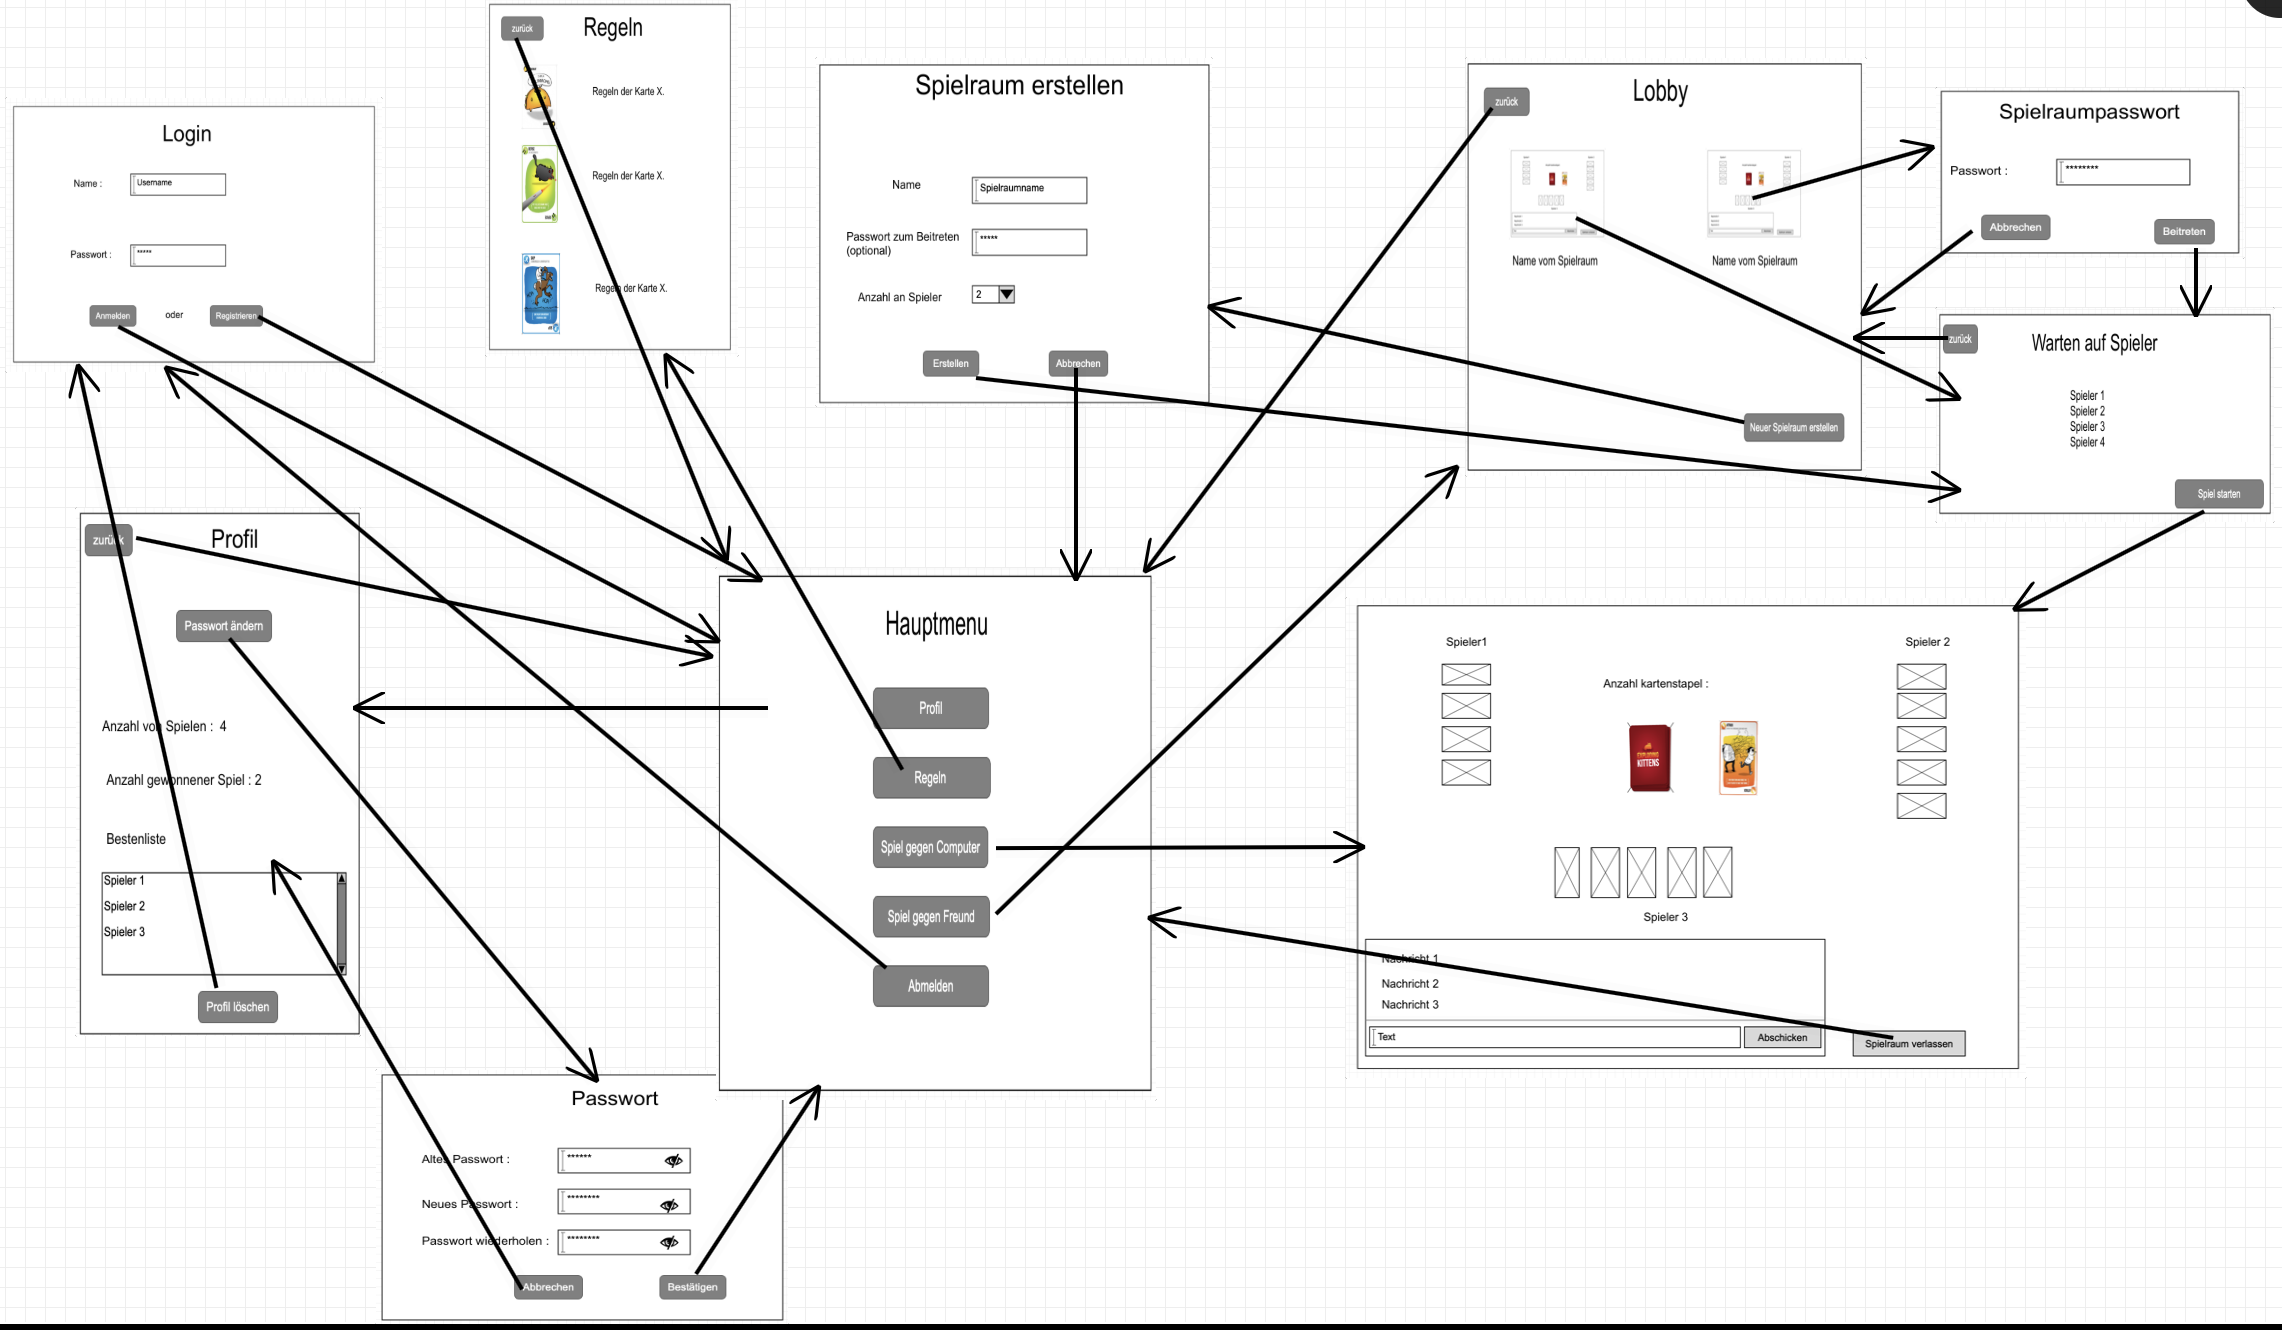
\includegraphics[width=0.9\textwidth]{img/Zusammenhang}
	\caption{Zusammenhang}
	\label{gui:zusammenhang}
\end{figure}